% !TEX root = ../main.tex
% !TEX program = xelatex
\section{问题一的模型建立与求解}
\subsection{电量流线性规划的建立}
问题一已知各时段的供需和电价，适合统筹全天安排。本文考虑峰谷电价策略、光伏空间预留策略和线性规划三种方案。前两种策略直观易用，但需要事先设置价格门槛或目标储电量；线性规划则能同时考虑当前充放电对后续用电的影响。由于费用和设备约束均为线性关系，本文采用\textbf{电量流线性规划}，并通过相同条件下的策略比较检验其效果。

\subsubsection*{（1）电量划分与决策变量}
沿用前文的144个10分钟时段。第 $k$ 段的负载电量和光伏电量为
\begin{equation}
E_k^L=L_k\Delta t,\qquad E_k^{PV}=P_k^{PV}\Delta t.
\label{eq:q1_energy}
\end{equation}
按照光伏优先满足负载的运行假设，定义
\begin{equation}
m_k=\min(E_k^L,E_k^{PV}),\qquad n_k=E_k^L-m_k,\qquad r_k=E_k^{PV}-m_k.
\label{eq:q1_gap_surplus}
\end{equation}
其中，$m_k$ 为光伏直接供电量，$n_k$ 为剩余负载缺口，$r_k$ 为富余光伏。

以外网充电量 $x_k$、光伏充电量 $y_k$、电池向负载输出的电量 $z_k$ 和时段末内部储电量 $S_k$ 为决策变量。电量分配关系如图~\ref{fig:q1_1}所示。

\begin{figure}[!htbp]
    \centering
    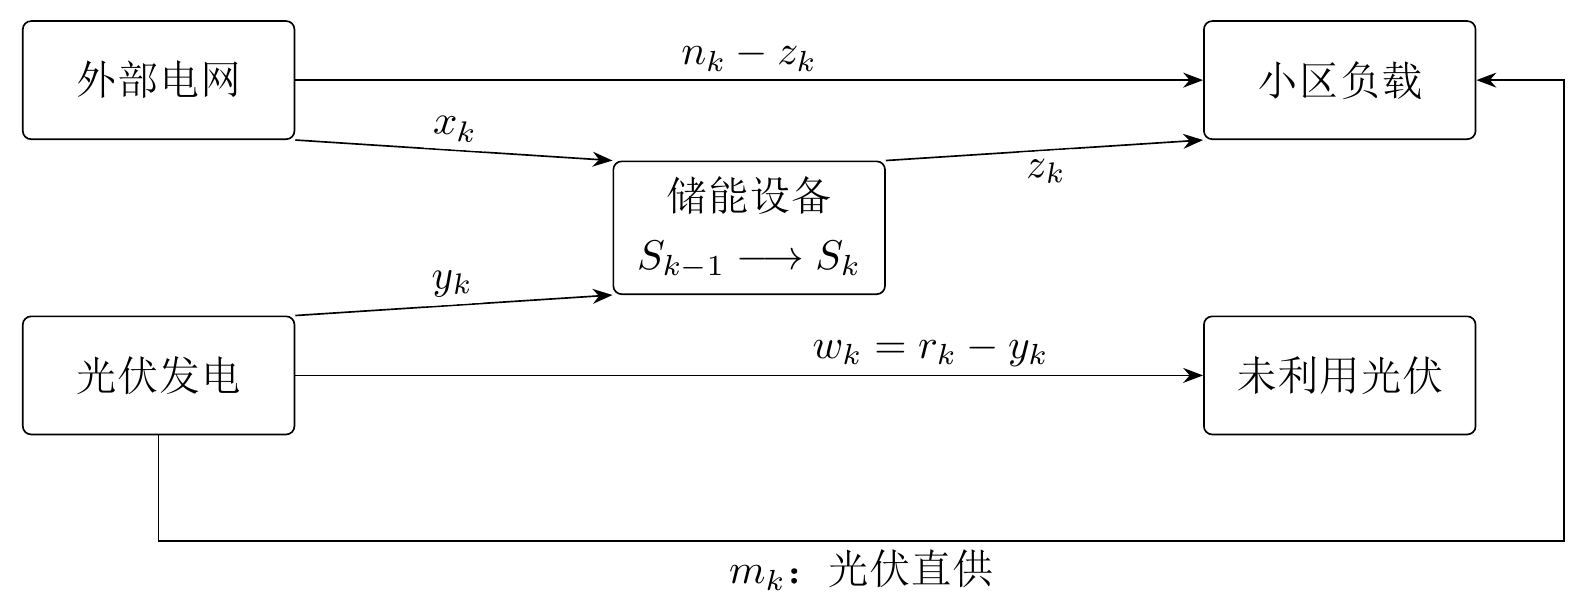
\includegraphics[width=0.95\textwidth]{fig/q1_1.png}
    \caption{问题一的电量分配关系}
    \label{fig:q1_1}
\end{figure}

外网既可补足负载缺口，也可给电池充电，购电量与未利用光伏电量为
\begin{equation}
q_k=n_k-z_k+x_k,\qquad w_k=r_k-y_k,
\label{eq:q1_purchase}
\end{equation}
其中，$q_k$ 为外网购电量，$w_k$ 为未利用光伏电量。

\subsubsection*{（2）目标函数}
以全天购电费用最低为目标：
\begin{equation}
\min C=\sum_{k=1}^{144}p_k(n_k-z_k+x_k).
\label{eq:q1_objective}
\end{equation}
该目标关注购电费用。即使储能损耗使总购电量有所增加，只要低价购电能够替代更昂贵的后续购电，仍可能降低总费用。

\subsubsection*{（3）约束条件}
\noindent\textbf{约束1：电量分配与供电限制。}光伏充电不超过富余量，电池放电不超过负载缺口：
\begin{equation}
x_k\ge0,\qquad 0\le y_k\le r_k,\qquad 0\le z_k\le n_k,
\label{eq:q1_supply_constraint}
\end{equation}
\noindent\textbf{约束2：充放电功率限制。}各时段充放电不超过设备允许功率：
\begin{equation}
x_k+y_k\le P_{\max}\Delta t,\qquad z_k\le P_{\max}\Delta t.
\label{eq:q1_power_constraint}
\end{equation}
其中，$P_{\max}\Delta t=5000/6\ \mathrm{kWh}$，计算时保留精确值。该限制作用于储能充放电，不限制外网直接向负载供电。

\noindent\textbf{约束3：储电量递推。}考虑充、放电各90\%的效率，内部储电量满足
\begin{equation}
S_k=S_{k-1}+\eta_c(x_k+y_k)-\frac{z_k}{\eta_d},\qquad \eta_c=\eta_d=0.9,
\label{eq:q1_soc_transition}
\end{equation}
\noindent\textbf{约束4：储电量上下限。}内部储电量保持在允许范围内：
\begin{equation}
S_{\min}\le S_k\le S_{\max},\qquad S_{\min}=1200,\quad S_{\max}=10800.
\label{eq:q1_soc_bound}
\end{equation}
\noindent\textbf{约束5：日初与日末电量相等。}两者均取6000 kWh：
\begin{equation}
S_0=S_{144}=6000.
\label{eq:q1_terminal_constraint}
\end{equation}
这样既保证储能在允许范围内运行，也避免通过消耗初始电量降低当天表面费用，使各策略能够在相同起点和终点下比较。

\subsection{模型求解}
模型包含576个连续变量，各时段通过储电量递推相互连接，采用SciPy的\texttt{linprog}接口调用HiGHS求解。

本题无需额外设置0—1变量区分充放电。若某时段同时充放电，则该段存在负载缺口，没有富余光伏，充电只能来自外网。取 $\delta=\min(x_k,z_k/0.81)>0$，将充电减少 $\delta$、放电减少 $0.81\delta$，不足的负载由外网直接补充。由于 $0.9\delta-0.81\delta/0.9=0$，储电变化不变，功率约束仍满足，而购电量减少 $0.19\delta$。电价为正时费用随之下降，因此最优解不会保留这种同时充放电。

\noindent\textbf{步骤1：整理时段供需。}按时间标签转换电量，计算光伏直供后的负载缺口和富余量。

\noindent\textbf{步骤2：求解购电与储能安排。}将时段供需和电价代入模型，求得购电、充放电和储电量。

\noindent\textbf{步骤3：核对并汇总结果。}复核供需、储能约束和费用，按模板时间标签填回结果。

\subsection{调度结果与策略比较}
\subsubsection*{（1）购电与储能结果}
线性规划得到全天购电量59482.70 kWh，购电费用\textbf{35126.85元}；储能累计充电20740.67 kWh、向负载输出16799.94 kWh。指定结果见表~\ref{tab:q1_purchase_result}和表~\ref{tab:q1_storage_result}，电量单位为kWh、费用单位为元。完整策略保存于\texttt{result1.xlsx}。

\begin{table}[!htbp]
    \centering
    \caption{微网在指定时间段的购电量及全天的购电量和购电费 }
    \label{tab:q1_purchase_result}
    \begin{tabular}{|c|c|c|c|c|c|}
        \hline
        时间段 & 购电量 & 时间段 & 购电量 & 时间段 & 购电量 \\
        \hline
        10:00-10:10 & 0.00 & 12:00-12:10 & 486.40 & 14:00-14:10 & 0.00 \\
        \hline
        16:00-16:10 & 394.93 & 18:00-18:10 & 636.98 & 20:00-20:10 & 0.00 \\
        \hline
        \multicolumn{2}{|c|}{全天购电量} & \multicolumn{1}{c|}{59482.70} & \multicolumn{2}{c|}{全天购电费} & \multicolumn{1}{c|}{\textbf{35126.85}}\\
        \hline
    \end{tabular}
\end{table}

\begin{table}[!htbp]
    \centering
    \caption{问题一各4小时区间的储能充放电量}
    \label{tab:q1_storage_result}
    \begin{tabular}{|c|c|c|c|c|c|}
        \hline
        时间段 & 充电量 & 放电量 & 时间段 & 充电量 & 放电量 \\
        \hline
        00:00--04:00 & 4500.00 & 0.00 & 04:00--08:00 & 833.33 & 5947.42 \\
        \hline
        08:00--12:00 & 3954.63 & 2121.42 & 12:00--16:00 & 6119.37 & 91.10 \\
        \hline
        16:00--20:00 & 0.00 & 5068.69 & 20:00--24:00 & 5333.33 & 3571.31 \\
        \hline
        \multicolumn{2}{|c|}{0:00储电量} & \multicolumn{1}{|c|}{6000.00} & \multicolumn{2}{c|}{24:00储电量} & \multicolumn{1}{c|}{6000.00}\\
        \hline
    \end{tabular}
\end{table}

表中充放电量按电池外侧计量，库存按内部电量计量。一个4小时区间同时出现充电和放电，表示不同10分钟时段采取了不同动作。

\subsubsection*{（2）策略比较}
峰谷策略按价格门槛安排充放电，光伏空间预留策略进一步为午间富余光伏保留储能空间。两种规则均比较27组参数：低价门槛取电价的15\%、25\%、35\%分位，高价门槛取65\%、75\%、85\%分位，目标储电量取6000、8400、10800 kWh。

分别选取已比较组合中费用最低的规则方案，与线性规划对照。各方案均在日末恢复6000 kWh，恢复库存所需的购电全部计入费用，结果见表~\ref{tab:q1_strategy_compare}。

\begin{table}[!htbp]
    \centering
    \caption{三种策略的全天购电费用比较}
    \label{tab:q1_strategy_compare}
    \begin{tabular}{cc}
        \toprule
        策略 & 全天购电费/元 \\
        \midrule
        峰谷电价策略 & 38276.64 \\
        光伏空间预留策略 & 37944.35 \\
        线性规划 & \textbf{35126.85} \\
        \bottomrule
    \end{tabular}
\end{table}

线性规划较峰谷策略节省3149.79元，降幅\textbf{8.23\%}；较光伏空间预留策略节省2817.50元，降幅\textbf{7.43\%}。三种策略的购电与储能安排如图~\ref{fig:q1_2}所示。

\begin{figure}[!htbp]
    \centering
    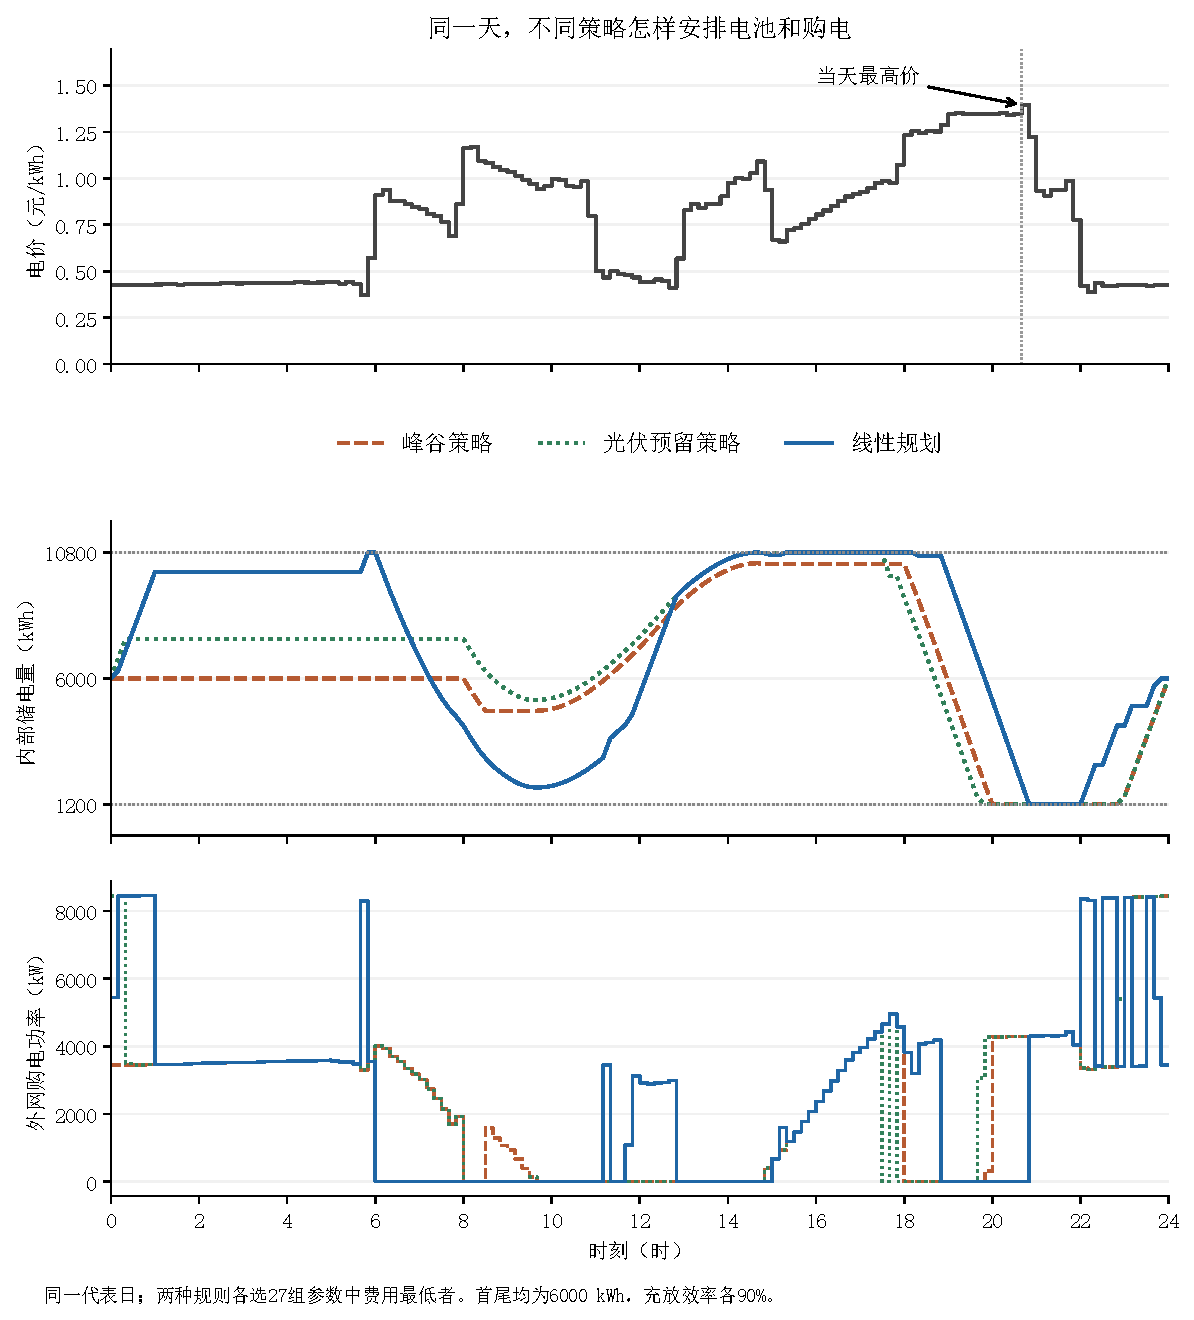
\includegraphics[width=0.73\textwidth]{fig/q1_daily_dispatch.pdf}
    \caption{三种策略在相同代表日下的购电与储能安排}
    \label{fig:q1_2}
\end{figure}

20:00时，两种规则策略均已降至1200 kWh的储电下限，线性规划仍保留5168.13 kWh。到20:40—20:50，电价达到全天最高的1.3952元/kWh，线性规划利用储能满足负载，外网购电量为零；另外两种策略则需购买715.65 kWh的高价电。

因此，全天统筹的优势在于\textbf{根据供需和价格变化，将有限储能留给更有价值的时段}。虽然线性规划因储能损耗多购电1740.28 kWh，但增加的低价购电替代了更昂贵的后续购电，最终费用更低。

\subsection{模型检验与初始电量分析}
逐时核对供需平衡、储电递推、容量与功率约束，并重新计算全天费用。三个初始电量案例的最大储电递推残差约为 $1.34\times10^{-12}\ \mathrm{kWh}$。利用对偶乘子独立重算费用下界后，求解费用与下界的最大差值约为 $1.22\times10^{-12}$ 元。两者均处于数值误差范围，支持所得解的可行性与数值最优性。

\begin{samepage}
将初始电量分别设为1200、6000和10800 kWh，并要求日末恢复原值，重新优化后的费用依次为35199.30、35126.85和35409.75元，前后两种状态较主方案增加0.21\%和0.81\%。
\par\end{samepage}

三种状态的费用相对主方案变化均不足1\%，且都为晚间最高价时段保留电量。这表明，主要调度规律对所比较初始储电量的变化较为稳定。
